\chapter{Ergebnisse}
In diesem Kapitel werden die Ergebnisse numerischer Experimente für das Schema aus Abschnitt \ref{sec:primal} vorgestellt. Tabelle \ref{tab:parameter} listet die einstellbaren Parameter mit einer kurzen Beschreibung und ihren Default-Werten auf.
\begin{table}
  \centering
  \caption{Einstellbare Parameter und ihre Default-Werte.}
  \label{tab:parameter}
  \sisetup{parse-numbers=false}
  \scriptsize
  \begin{tabular}{
% format 1.3 bedeutet eine Stelle vorm Komma, 3 danach
    l
    l
    l
  }
    \toprule
    {Formelzeichen} & Beschreibung & Default-Wert \\
    \midrule
       & \emph{Physikalische Parameter} & \\
    $L_x (L_y)$ &Länge des Rechengebietes in $x$- ($y$-) Richtung & $\SI{106}{\nano\meter}$ $(\SI{130}{\nano\meter})$ \\
    $L_D$ & Ausdehnung des Spannungsabfalls (s. Abbildung \ref{fig:pot1}) & $\SI{26}{\nano\meter}$\\
    $L_1$ & Abstand der Potentialbarrieren (s. Abbildung \ref{fig:pot1}) &$\SI{6}{\nano\meter}$ \\
    $L_2$ & Breite der Potentialbarrieren  (s. Abbildung \ref{fig:pot1}) &$\SI{4}{\nano\meter}$ \\
    $V_0$ & Barrierenhöhe (Differenz der Leitungsbandkantenenergien) &$\SI{0.2098}{\electronvolt}$ \\
    $N_D$ & Donatorkonzentration des GaAs & $10^{24}\,\text{m}^{-3}$ \\
    $m$ & Effektive Elektronenmasse in GaAs & $0,063 m_e$ \\
    $\mu$   & Chemisches Potential (wird errechnet, siehe Abschnitt \ref{sec:A_3}) & $\SI{46}{\milli\electronvolt}$ \\
    $\delta$ & Einflussbereich des ac{cap}, siehe Gleichung \eqref{eq:cap} & $0,2 L_y$\\
    $W_0$ & Stärke des \ac{cap}, siehe Gleichung \eqref{eq:cap} &$-1V_0$ \\
    $U$   &Spannung, die über die Strecke $L_D$ abfällt & $\SI{0}{\volt}$ \\
    \midrule
     & \emph{Parameter der Numerik} & \\
    $K_x$ & \# Zellen der \ac{dg}-Diskretisierung & 60 \\
    $K_y$ & \# Zellen der \ac{fv}-Diskretisierung & 100 \\
    $N$ & Polynomgrad der \ac{dg}-Diskretisierung & 2 \\
    $N_q$ & Quadraturordnung für Methode G2 & 20 \\
    $\kappa$ & Strafparameter des numerischen Flusses, siehe Gleichung \eqref{eq:numflux} &$\nicefrac{1}{2}$ \\
    \midrule
     & \emph{Parameter des Programmablaufs} & \\
    doGL & Soll Methode G2 verwendet werden?(sonst G1) & true \\
    doPotConv & Soll das Potential mit einer Gaußverteilung gefaltet werden? & false\\
    withCAP & Soll das \ac{cap} eingeschaltet werden? & true \\
    doTransient & Soll transient gerechnet werden? & false \\
    doGummel & Soll selbstkonsistent gemäß den Erläuterungen in Kapitel \ref{sec:A_4} gerechnet werden? \\
    Nrefine  & \# Verfeinerungen in der Polynomordnung $N$ mit $N_{i+1}=N_i+1$ & 0 \\
    Krefine  & \# Verfeinerungen in der Anzahl Elemente $K_x$ mit $K_{x,i+1}=2K_{x,i}$ & 0 \\
    \bottomrule
  \end{tabular}
\end{table}
Offenbar entsteht eine große Variationsmöglichkeit. Zunächst soll jedoch im nächsten Abschnitt die Funktionalität des Schemas getestet werden für ein analytisch lösbares Randwertproblem. Daraufhin wird die stationäre Lösung näher untersucht. Der mit der Elektronendichte korrespondierende Realteil sowie der mit dem Strom korrespondierende Imaginärteil werden für verschiedene Spannungen gezeigt. Aus einer Mittelung des Stromes über $x$ ergibt sich der Gesamtstrom in Abhängigkeit von der Spannung. Hierfür soll in Kapitel \ref{sec:IV} insbesondere der Einfluss der physikalischen Längen sowie die Übereinstimmung mit der Erwartung gemäß Abbildung \ref{fig:IVkurve} untersucht werden. Besonders interessant sind darüber hinaus Fehlerraten, die eine Aussage über die Qualität des verwendeten Verfahrens liefern. Dazu wird in Kapitel \ref{sec:rates} einerseits ein Vergleich mit der \ac{tf} aus Kapitel \ref{sec:TFmethod} gezogen, andererseits eine iterative Fehlerrate definiert. Abgeschlossen wird das Kapitel durch eine Untersuchung der transienten Lösung in Abschnitt \ref{sec:transient}.

\section{Notation}\label{sec:notation_4}
Für numerische Untersuchungen ist die Definition eines \emph{analytischen Fehlers} \index{analytischer Fehler}
\begin{equation}
  e_{\nicefrac{i}{r}}^{\alpha} = \norm{\nicefrac{\operatorname{Re}}{\operatorname{Im}} (u - u\fin^{\alpha})}_{L^2(\Omega)}
  \label{eq:error_ana}
\end{equation}
sowie eines \emph{iterativen Fehlers}\index{iterativer Fehler}
\begin{equation}
  e_{\mathcal{T}, \nicefrac{i}{r}}^{\alpha} = \norm{\nicefrac{\operatorname{Re}}{\operatorname{Im}} (u\fin^{\alpha} - u\fin^{\alpha-1})}_{L^2(\Omega)}
\end{equation}
sinnvoll, wobei $\Omega=\Omega_x \times \Omega_y$ das Rechengebiet, $u$ die exakte Lösung und $u\fin$ die Ritz-Approximation sind. Der Index $\alpha>0$ bezieht sich auf die Verfeinerung des Gitters in $x$-Richtung gemäß $K_x^{\alpha} = 2^\alpha$. Wenn nicht anders angegeben, werden die benötigten Integrale in $x$-Richtung mit Gauß-Lobatto Quadratur der Ordnung $N$ (also gleich der Ordnung des \ac{dg}-Verfahrens) berechnet.
In $y$-Richtung hingegen wird schlicht $\int_{\Omega_y}\diff y f(y) \approx \sum_{j=1}^{K_y} h_y f(y_j)$ berechnet, da $f(y)$ im \ac{fv}-Verfahren konstant ist innerhalb der Zelle $j$.

Für die Betrachtung der \emph{Konvergenzordnung}\index{Konvergenzordnung} in Abschnitt \ref{sec:rates} werden ferner die Fehlerraten
\begin{equation}
\begin{aligned}
  r_{\nicefrac{i}{r}}^{\alpha} &= \frac{\ln(e_{\nicefrac{i}{r}}^{\alpha}) - \ln(e_{\nicefrac{i}{r}}^{\alpha-1})}{\ln(K_x^{\alpha-1}) - \ln(K_x^{\alpha})} \qquad\text{und}\\
  r_{\mathcal{T},\nicefrac{i}{r}}^{\alpha} &= \frac{\ln(e_{\mathcal{T},\nicefrac{i}{r}}^{\alpha}) - \ln(e_{\mathcal{T},\nicefrac{i}{r}}^{\alpha-1})}{\ln(K_x^{\alpha-1}) - \ln(K_x^{\alpha})}
\end{aligned}
  \label{eq:fehlerraten}
\end{equation}
definiert. Daraus lassen sich noch $r_{\nicefrac{i}{r}}$ bzw. $r_{\mathcal{T},\nicefrac{i}{r}}$ als Mittelwerte über $\alpha$ errechnen. Die Definition der Fehlerrate ist motiviert durch eine Fehlerabschätzung der Form $e \leq ch_x^r$. Logarithmieren und Subtrahieren für zwei verschiedene Gitterabstände $h_x$ liefert die Konvergenzordnung $r$.

Wann immer die numerische Lösung $u\fin$ ausgwertet werden muss, sind die Gleichungen\eqref{eq:ellPsi} und \eqref{eq:vandermonde} hilfreich. Sei nun $u\fin$ an der Stelle $x_0$ auszuwerten. Dann ist zunächst das Element $D^k$ zu suchen, für das $x_0\in D^k$ gilt. Durch Gleichung \eqref{eq:affmap} ergibt sich hieraus $r_0$ als Koordinate auf dem Referenzelement $I$. Dann gilt nach Gleichung \eqref{eq:nodal}
\begin{align*}
  v\fin(x_0) &= v\fin^k(r_0,t) = \sum_{j=1}^{N_p} v_{\mathcal{T},j}^k(t)\ell_j(r_0) \\
   &\stackrel{\eqref{eq:ellPsi}}{=} \sum_{j=1}^{N_p} v_{\mathcal{T},j}^k(t) ((\van^T)^{-1}\Psi(r_0))_j \; .
\end{align*}
Jetzt wird eine weitere Vandermondematrix $\tilde{\van}$ der Dimension $1\times N_p$ eingeführt, um den Punkt $r_0$ zu errechnen. Nach Gleichung \eqref{eq:vandermonde} ist also $\tilde{\van}_{1j}=\Psi_j(r_0)$. Dann folgt
\begin{align*}
  v\fin(x_0) &= \sum_{i=j}^{N_p} v_{\mathcal{T},j}^k(t) ((\van^T)^{-1}\tilde{\van}^T)_{j,1} \\
  &= (\tilde{\van}\van^{-1})\underline{v}_j^k(t) \; ,
\end{align*}
wobei im letzten Schritt die Definition \ref{def:matrizen} sowie die Vertauschbarkeit von Invertierung und Transponierung einer Matrix eingegangen sind. Falls $r_0\in\{-1,1\}$, so ist $u\fin$ auf einer Kante auszuwerten. An diesen Stellen wird der numerische Fluss verwendet. Anhand des Vorzeichens des zu $y_j$ korrespondierenden Eigenwerts $\lambda_j$ aus Gleichung \eqref{eq:Lambda} wird entweder $u\fin^+$ oder $u\fin^-$ ausgewertet, siehe auch Abbildung \ref{fig:notation_DG}.

Die soeben angestellten Überlegungen zur Auswertung der numerischen Lösung mögen aufwändig erscheinen. Wenn jedoch Fehlerraten bestimmt werden sollen, ist die exakte Auswertung nach Ansicht des Autors unerlässlich. Eine interpolatorische Bestimmung der $L^2$-Norm führt ansonsten zu Abweichungen. Insbesondere für grobe Diskretisierungen (also kleine Werte von $K_x$, $N$) sind diese deutlich zu spüren.

\section{Test für ein analytisch lösbares Randwertproblem}\label{sec:test}
Losgelöst von der physikalischen \ac{lvn} wird in diesem Abschnitt für Testzwecke die Gleichung \eqref{eq:qschema} mit
\begin{equation*}
  \begin{aligned}
    A^y& = 0 \\
    B^y_{j,j} &= -1/a(y_j) \qquad \text{mit} \;\; a(y)=\sin\left(\frac{2\pi y}{L_y}\right) \\
    C^y_{j,j} &= i
  \end{aligned}
\end{equation*}
mit äquidistanten $y_1,\dots,y_{K_y}=-L_y/2,\dots,L_y/2$ betrachtet. Unter den Randbedingungen
\begin{equation*}
  \begin{aligned}
    u(x,y)|_{\partial \Omega} = \exp(ia(y)x)
  \end{aligned}
\end{equation*}
entspricht die analytische Lösung der Gleichung \eqref{eq:qschema} eben dieser Funktion, also $u(x,y) = \exp(ia(y)x)$ auf ganz $\Omega$. Für die diagonalisierte Gleichung \eqref{eq:diagLVN} ist mit $v_t=0$ die Geschwindigkeit $\Lambda^y=B^y$ und der Driftoperator $G=C^y$. Die Systemmatrix aus Abschnitt \ref{sec:implementierung} wird entsprechend angepasst.

Nun liegt der sehr einfache Fall von $K_y$ entkoppelten Advektions-Reaktions Gleichungen vor. Aus der umfangreichen Literatur kann beispielsweise in \cite{lesaint1974finite} die \emph{a priori} Fehlerabschätzung
\begin{equation}
  e \leq c h_x^{N_x + 1} \label{eq:optimaleKonvergenz}
\end{equation}
gefunden werden, falls $u \in H^{N_x+2}$ liegt, was für die obige Lösung in der Tat gilt. Diese Konvergenzordnung ist optimal und lediglich für reinen Upwind Fluss in linearen Problemen gültig. Die Abbildung \ref{fig:testResult} zeigt die im vorherigen Abschnitt definierten Fehler in Abhängigkeit von Polynomgrad und Anzahl der Elemente.
\begin{figure*}
    \centering
    \begin{subfigure}[b]{0.475\textwidth}
        \centering
        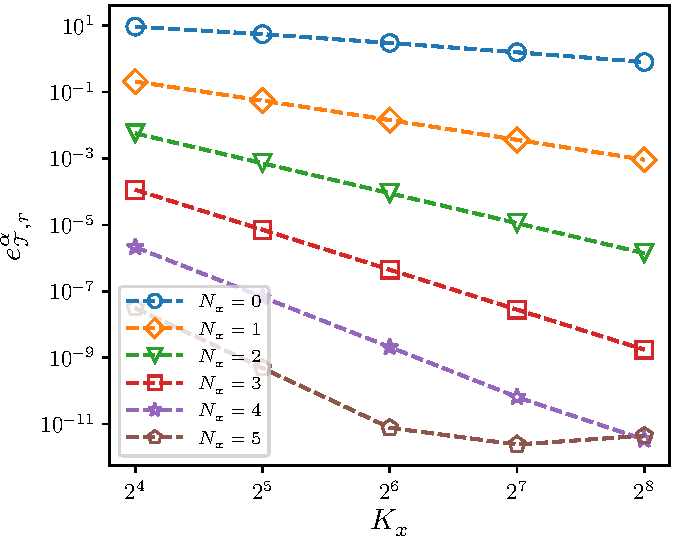
\includegraphics[width=\textwidth]{plots/test1_r.pdf}
        \caption[]%
        {{\small Analytischer Fehler $e_r$.}}
    \end{subfigure}
    \hfill
    \begin{subfigure}[b]{0.475\textwidth}
        \centering
        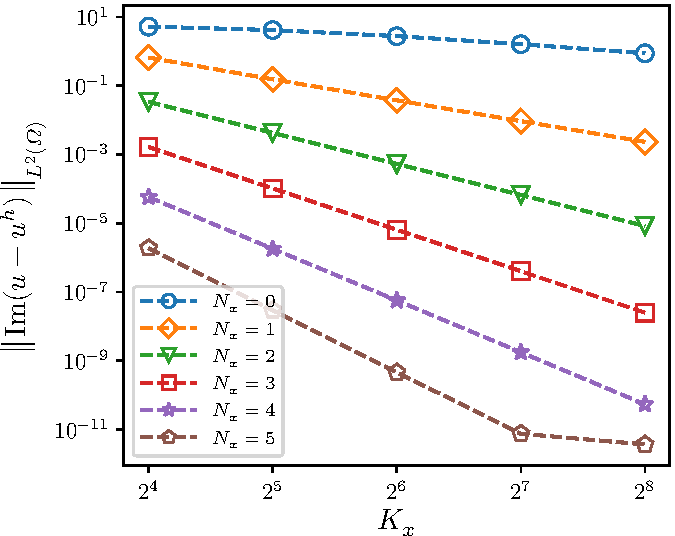
\includegraphics[width=\textwidth]{plots/test1_i_rel.pdf}
        \caption[]%
        {{\small Iterativer Fehler $e_{\mathcal{T},i}$.}}
    \end{subfigure}
    \caption[]
    {Fehler in Abhängigkeit von Polynomgrad $N$ und Anzahl Elemente $K_x=2^{\alpha}$ mit $K_y=50$. Die Steigung der Geraden stellt die Fehlerrate dar, welche hier optimal ist. Bei $e\approx10^{-11}$ ist offenbar die CPU-Genauigkeit erreicht.}
    \label{fig:testResult}
\end{figure*}
Es zeigt sich optimale Konvergenz nach Gleichung \eqref{eq:optimaleKonvergenz} mit
\begin{align*}
  r_r &= \{0.86\pm0.07,\; 1.94\pm0.03,\; 3.0\pm0.0,\; 4.0\pm0.0,\; 5.0\pm0.0,\; 4.55\pm2.04\} \\
  r_i &= \{0.83\pm0.08, 1.95\pm0.03, 3.0\pm0.0, 4.0\pm0.0, 5.0\pm0.0, 4.6\pm1.97\} \\
  r_{\mathcal{T},r} &= \{0.63\pm0.16, 2.06\pm0.05, 3.0\pm0.0, 4.0\pm0.0, 5.0\pm0.0, 5.97\pm0.04\} \\
  r_{\mathcal{T},i} &= \{0.57\pm0.18,\; 2.05\pm0.04,\; 3.0\pm0.0,\; 4.0\pm0.0,\; 5.0\pm0.0,\; 5.97\pm0.04\}
\end{align*}
jeweils für $N=\{0,\dots,5\}$. Imaginärteil und Realteil zeigen keine erkennbaren Unterschiede auf. Der Einbruch für feine Diskretisierungen ist der endlichen CPU-Genauigkeit zuzuschreiben.

\section{Observablen der stationären Lösung}\label{sec:IV}
Die in Kapitel \ref{sec:2_1} eingeführten Observablen der Teilchendichte $n(x,t)$ nach Gleichung \eqref{eq:expval_n} und der Stromdichte $j(x,t)$ nach Gleichung \eqref{eq:expval_j} lassen sich aus der Dichtematrix auf einfache Weise gewinnen. Für die Stromdichte wird noch eine Ableitung bezüglich $y$ benötigt. Hierfür wird der Differenzenquotient gemäß
\begin{equation*}
  \partial_y u\fin(x,y,t)|_{y=0} = \frac{1}{h_y}(u\fin(x,y_{K_y/2+1},t)-u\fin(x,y_{K_y/2},t))
\end{equation*}
gebildet. Da $K_y$ stets gerade gewählt wird, liegt die Kante zwischen den Elementen $K_y/2+1$ und $K_y/2$ genau bei $y=0$.

\subsection{Dichtematrix}
Ein erster Test des Verfahrens überprüft die Symmetrieeigenschaften der numerischen Lösung. Mit Hilfe von Gleichung \eqref{eq:Liouvilleoperator} ist in Kapitel \ref{sec:dynamik} gezeigt worden, dass die exakte Lösung im stationären Fall $u(x,y) = -u^*(x,-y)$ erfüllt. Die Differenz $(u\fin(x,y)-u\fin^*(x,-y))/\norm{u\fin(x,y)}_{L^2(\Omega)}$ ist in Abbildung \ref{fig:parity} gezeigt.
\begin{figure}
  \centering
  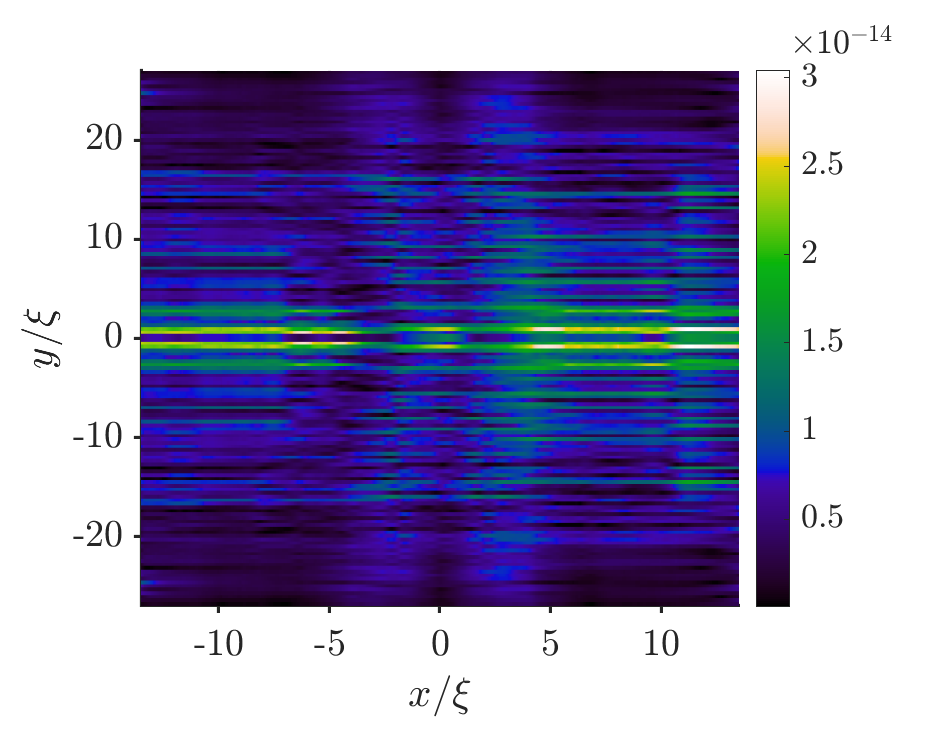
\includegraphics[width=1.0\textwidth]{plots/parity_abs.eps}
  \caption{Die Symmetrieanforderung $u\fin(x,y)-u\fin^*(x,-y) = 0$ wird bis auf CPU-Genauigkeit erfüllt.}
  \label{fig:parity}
\end{figure}

Abbildung \ref{fig:solution} zeigt Real- und Imaginärteil der numerischen Lösung für zwei Spannungen $U_1=\SI{0}{\volt}$, $U_2=\SI{0.14}{\volt}$.
\begin{figure*}
    \centering
    \begin{subfigure}[b]{0.48\textwidth}
        \centering
        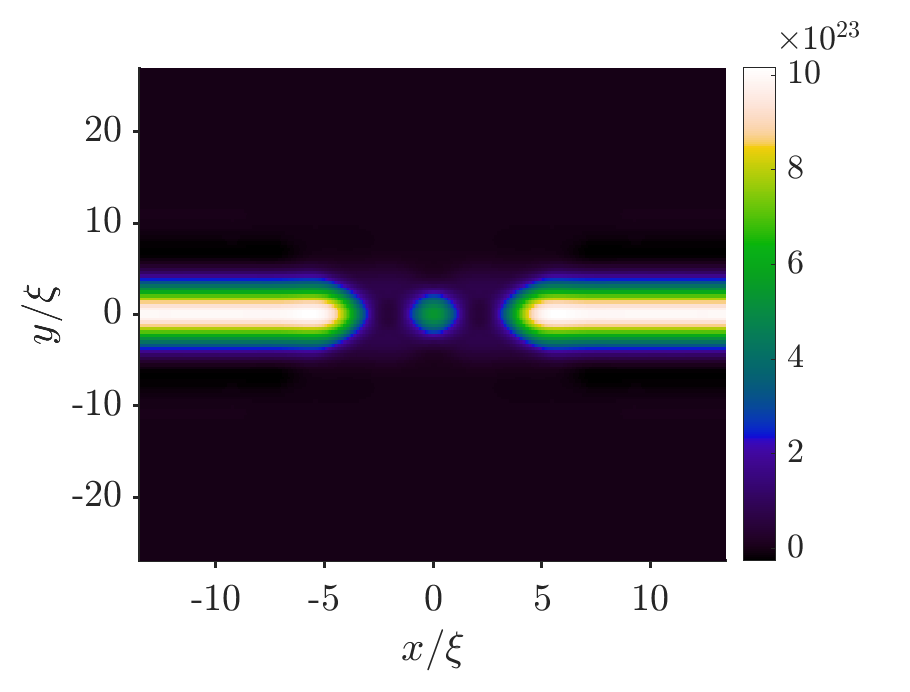
\includegraphics[width=\textwidth]{plots/section2/real_0.00V_Kx30_Nx4_Ky150_flat.eps}
        \caption[]%
        {{\small Realteil bei $U_1=\SI{0}{\volt}$.}}
        % \label{fig:G_1}
    \end{subfigure}
    \hfill
    \begin{subfigure}[b]{0.48\textwidth}
        \centering
        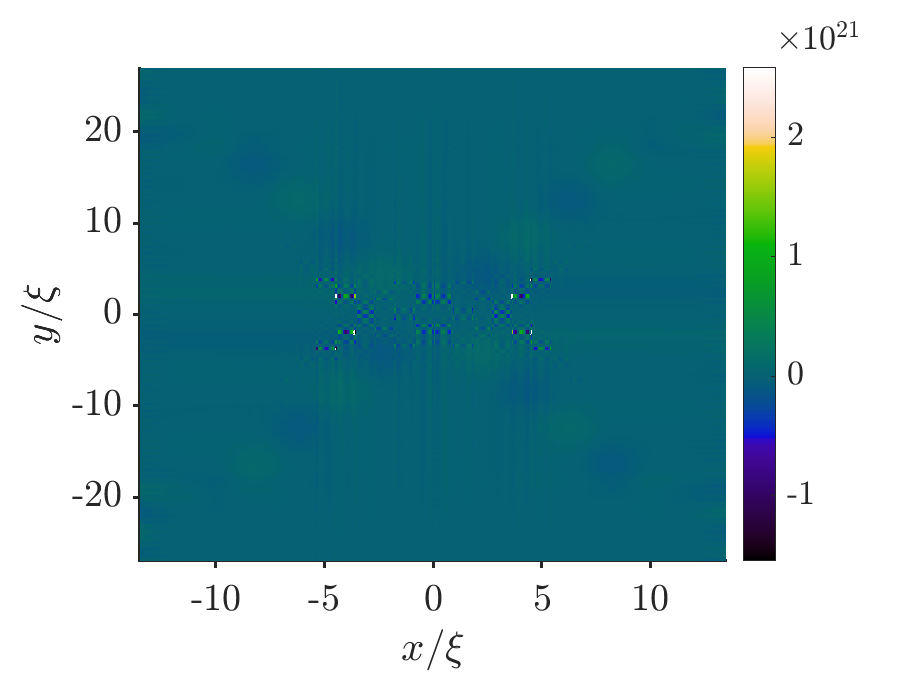
\includegraphics[width=\textwidth]{plots/section2/imag_0.00V_Kx30_Nx4_Ky150_flat.eps}
        \caption[]%
        {{\small Imaginärteil bei $U_1=\SI{0}{\volt}$.}}
        % \label{fig:G_2}
    \end{subfigure}
    \vskip\baselineskip
    \begin{subfigure}[b]{0.48\textwidth}
        \centering
        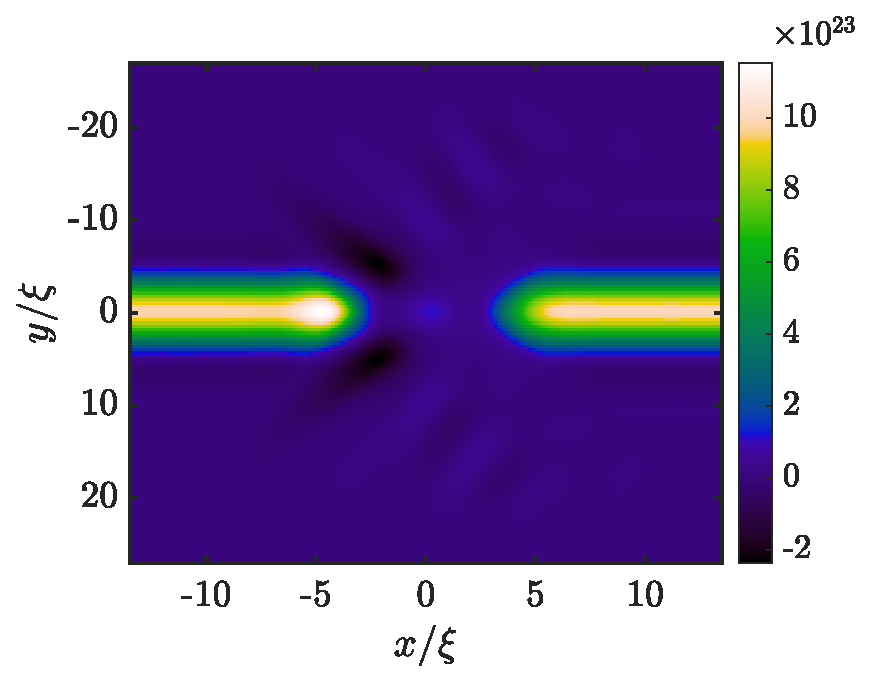
\includegraphics[width=\textwidth]{plots/section2/real_0.14V_Kx30_Nx4_Ky150_flat.eps}
        \caption[]%
        {{\small Realteil bei $U_2=\SI{0.14}{\volt}$.}}
        % \label{fig:G_3}
    \end{subfigure}
    \quad
    \begin{subfigure}[b]{0.48\textwidth}
        \centering
        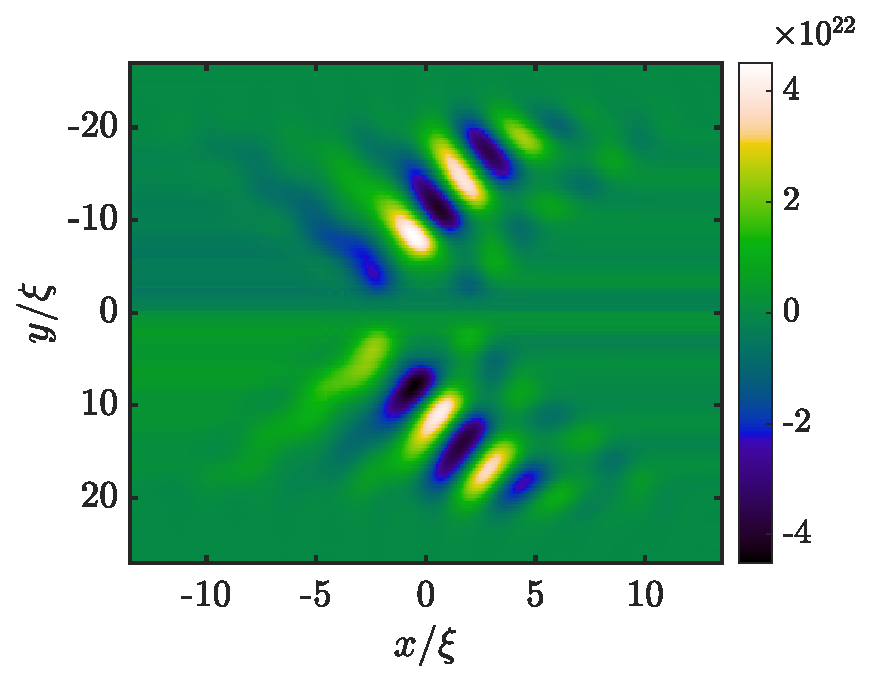
\includegraphics[width=\textwidth]{plots/section2/imag_0.14V_Kx30_Nx4_Ky150_flat.eps}
        \caption[]%
        {{\small Imaginärteil bei $U_2=\SI{0.14}{\volt}$.}}
        % \label{fig:G_4}
    \end{subfigure}
    \caption[]
    {Numerische Lösung für zwei verschiedene Spannungen, aufgeteilt in Imaginär- und Realteil. Parameter der Numerik: $K_x=30$, $N=4$, $K_y=150$. Physikalische Parameter: $L_x=\SI{66}{\nano\meter}$. Die Lösung wird an $400\times400$ äquidistant verteilten Punkten exakt ausgewertet.}
    \label{fig:solution}
\end{figure*}
Zum Vergleich ist in Abbildung \ref{fig:solution_gummel} das analoge Ergebnis einer selbstkonsistenten Rechnung (vgl. Kapitel \ref{sec:A_4}) zu sehen.
\begin{figure*}
    \centering
    \begin{subfigure}[b]{0.48\textwidth}
        \centering
        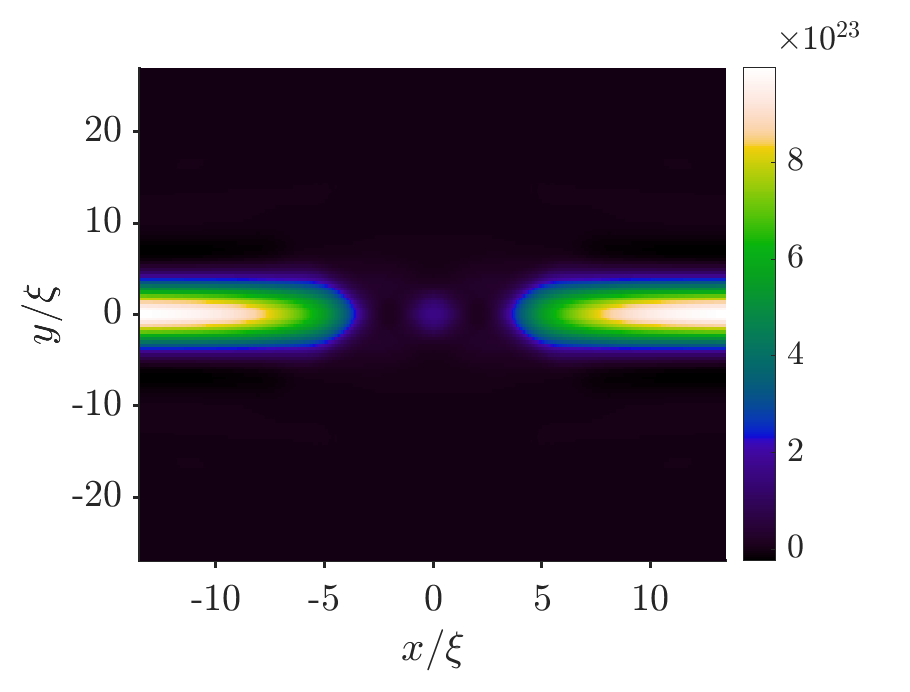
\includegraphics[width=\textwidth]{plots/section2/real_0.00V_Kx30_Nx4_Ky150_gummel_flat.eps}
        \caption[]%
        {{\small Realteil bei $U_1=\SI{0}{\volt}$.}}
        % \label{fig:G_1}
    \end{subfigure}
    \hfill
    \begin{subfigure}[b]{0.48\textwidth}
        \centering
        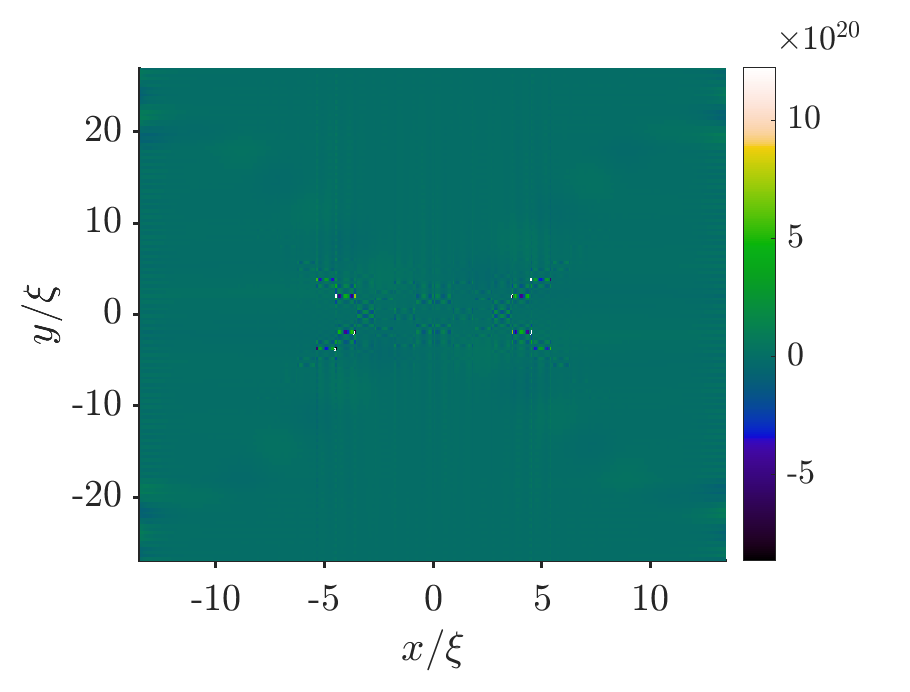
\includegraphics[width=\textwidth]{plots/section2/imag_0.00V_Kx30_Nx4_Ky150_gummel_flat.eps}
        \caption[]%
        {{\small Imaginärteil bei $U_1=\SI{0}{\volt}$.}}
        % \label{fig:G_2}
    \end{subfigure}
    \vskip\baselineskip
    \begin{subfigure}[b]{0.48\textwidth}
        \centering
        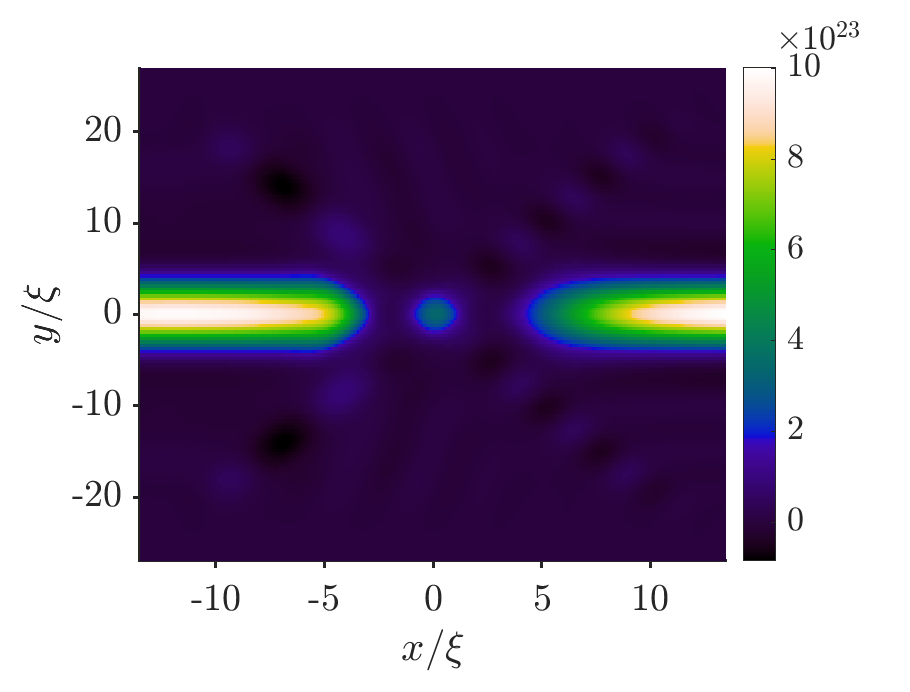
\includegraphics[width=\textwidth]{plots/section2/real_0.14V_Kx30_Nx4_Ky150_gummel_flat.eps}
        \caption[]%
        {{\small Realteil bei $U_2=\SI{0.14}{\volt}$.}}
        % \label{fig:G_3}
    \end{subfigure}
    \quad
    \begin{subfigure}[b]{0.48\textwidth}
        \centering
        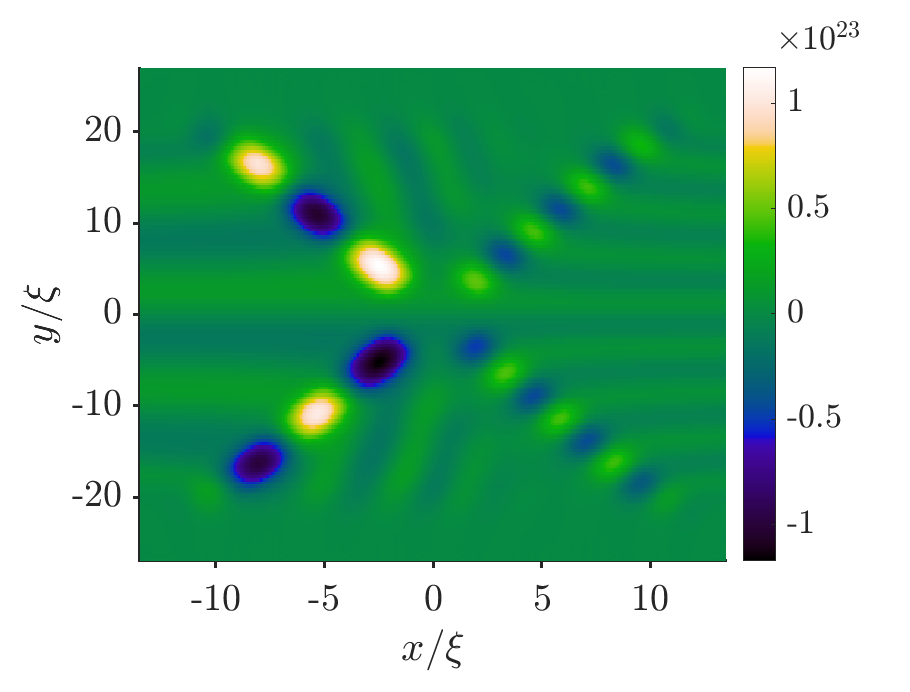
\includegraphics[width=\textwidth]{plots/section2/imag_0.14V_Kx30_Nx4_Ky150_gummel_flat.eps}
        \caption[]%
        {{\small Imaginärteil bei $U_2=\SI{0.14}{\volt}$.}}
        % \label{fig:G_4}
    \end{subfigure}
    \caption[]
    {Selbstkonsistente Rechnung mit ansonsten gleichen Parametern wie in Abbildung \ref{fig:solution}.}
    \label{fig:solution_gummel}
\end{figure*}
Die gezeigten Ergebnisse decken sich qualitativ mit den Ergebnissen anderer Verfahren wie einem \ac{FV}/\ac{FV}-Hybridverfahren in \cite{lukas1} oder einem Upwind-Differenzen-Schema für die Wignergleichung wie in \cite{frensley2}. Ein quantitativer Vergleich wird in Kapitel \ref{sec:rates} mit Hilfe der \ac{tf} aus Kapitel \ref{sec:TFmethod} vorgenommen. Ein Nachteil zeigt sich für den Imaginärteil im Gleichgewichtsfall bei $U_1=\SI{0}{\volt}$. Andere Verfahren (\ac{qtbm} und \ac{tf}) legen nahe, dass der Imaginärteil bis auf CPU-Genauigkeit verschwinden sollte, was hier nicht bestätigt werden kann.
Feinere Diskretisierungen verbessern zwar die Resultate diesbezüglich, jedoch konnte aufgrund begrenzter Rechenkapazität ein nomineller Unterschied zwischen Real- und Imaginärteil von ca. vier Größenordnungen nicht überschritten werden. Hier zeigt sich bereits, dass bezüglich des Imaginärteils eine Fehlerrate nach Gleichung \eqref{eq:optimaleKonvergenz} nicht erwartet werden kann.

\subsection{Strom-Spannungs-Kennlinien}
Für einen qualitativen Vergleich werden im Folgenden Ergebnisse einer \ac{qtbm}-Rechnung mit einbezogen. Da die selbstkonsistente Rechnung für angelegte Spannungen keine gute Konvergenz zeigt, beschränken sich die Berechnungen auf Flachband-Modelle gemäß Abbildung \ref{fig:pot1}.

\begin{figure}
  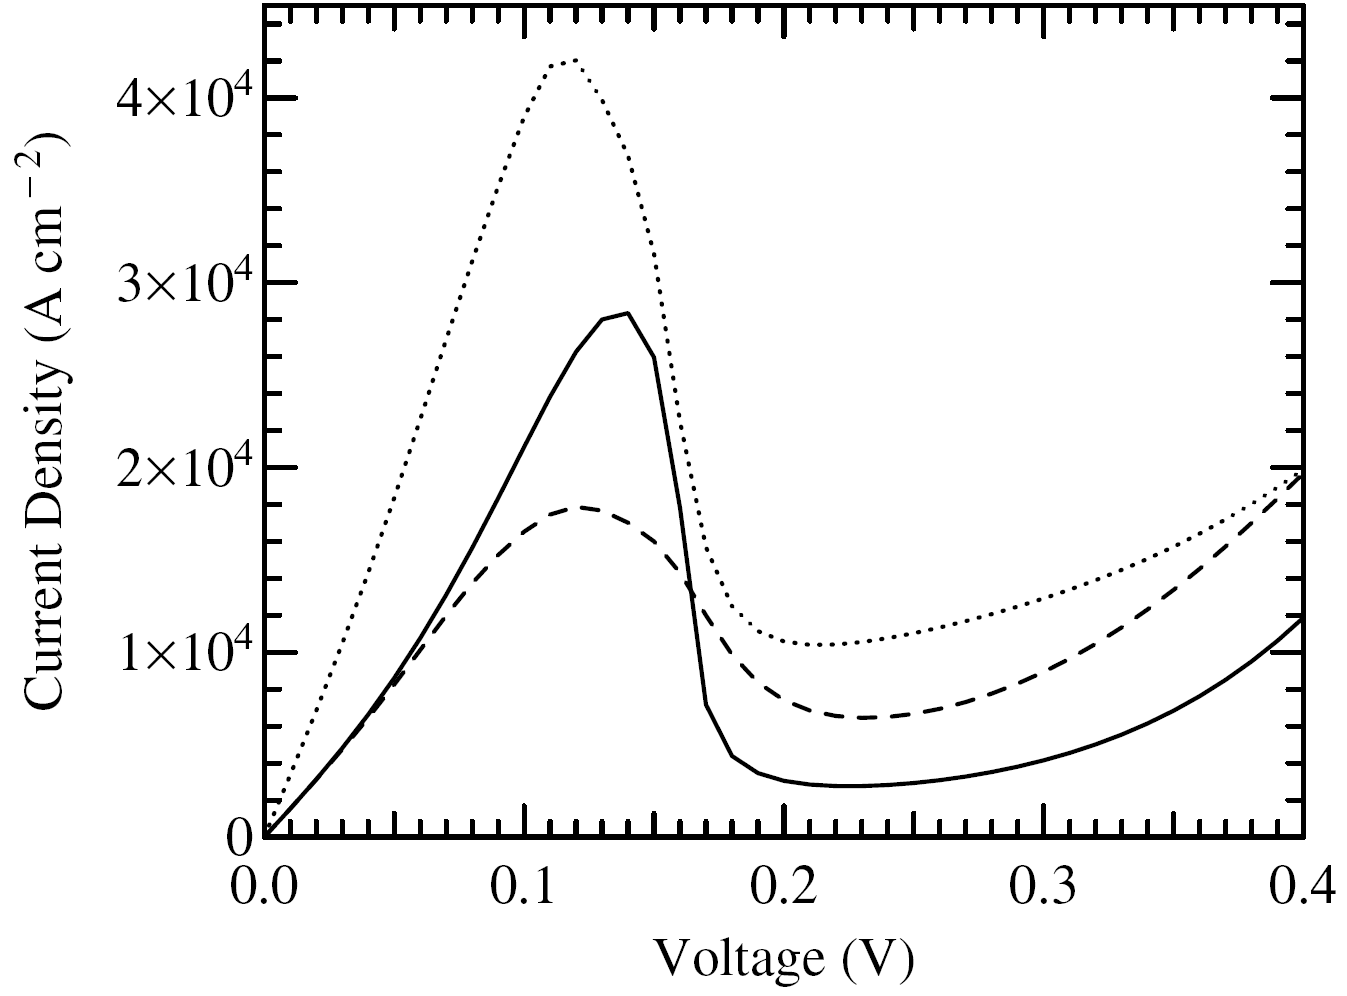
\includegraphics{plots/frensley.png}
  \caption{aus frensley_quantentransport.pdf}
  \label{}
\end{figure}

- IV Kurven für verschiedene Längen Lr, Lq sowie Gummel/ohne Gummel

\section{Konvergenzordnung der stationären Lösung}\label{sec:rates}


\section{Transiente Lösung}\label{sec:transient}
